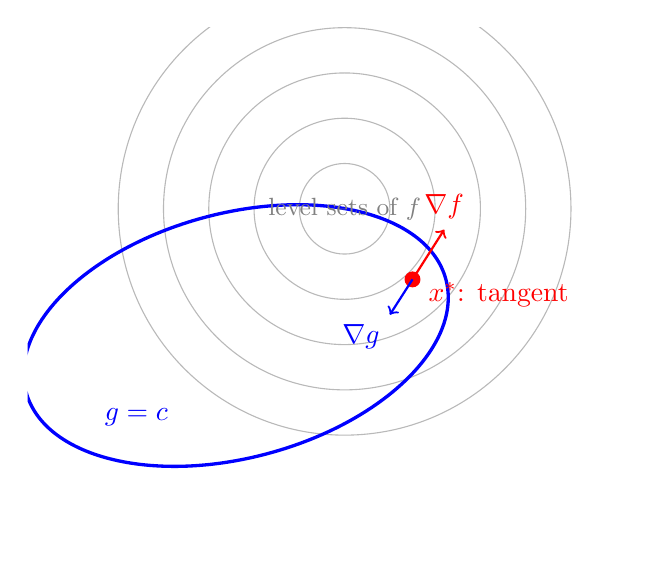
\begin{tikzpicture}[scale=1.15]
% level sets of f (circles about (3,3)) and constraint g = circle x^2+y^2=1-ish ellipse
\begin{scope}
\clip (-0.3,-0.4) rectangle (6.4,5.4);
\foreach \r in {0.5,1.0,1.5,2.0,2.5}
  \draw[gray!55] (3.2,3.4) circle (\r);
\draw[very thick,blue] (2.0,2.0) ellipse [x radius=2.4,y radius=1.35,rotate=15];
% the tangency point: level set kissing the constraint
\fill[red] (3.95,2.62) circle (2.5pt);
\node[red] at (4.9,2.45) {$x^{*}$: tangent};
% gradient arrows at tangency: parallel
\draw[->,thick,red] (3.95,2.62) -- ++(0.35,0.55) node[above]{$\nabla f$};
\draw[->,thick,blue] (3.95,2.62) -- ++(-0.25,-0.39) node[below left]{$\nabla g$};
\node[blue] at (0.9,1.1) {$g=c$};
\node[gray] at (3.2,3.4) {\small level sets of $f$};
\end{scope}
\end{tikzpicture}
